\newif\ifPAPER  
\PAPERtrue % select either slide or note
%\PAPERfalse  

\def\g4{{\sf Geant4}}

\newcommand{\codeAlgorithm}[1]{
\addcontentsline{toc}{section}{Résumé}
\begin{center}\fbox{\parbox{12cm}{\bf #1}}\end{center}}

\newcommand{\cppintro}[1]{
\lstset{language=C,
caption= #1 ,
label=listing:boundary}}

\def\cppstart{\begin{lstlisting}}
\def\cppend{\end{lstlisting}}

\newif\ifCITENOTE 
\CITENOTEtrue

\ifPAPER
\documentclass[twoside,floatfix,a4wide]{d}
\usepackage{multirow}
\usepackage{url}
\usepackage{listings}
\usepackage{graphicx}
\usepackage{wrapfig}
%\usepackage{makeidx}
\usepackage{subfig}
\usepackage{fancyhdr}
%\usepackage{asymptote}
\usepackage{amsmath}
\usepackage{verbatim} % for comment
\usepackage{eurosym} 
\usepackage{color} % for definecolor
\usepackage[colorlinks,bookmarks=true]{hyperref}

\numberwithin{equation}{section} % reguires amsmath-package
\pagestyle{fancy}
\fancyhead{} % clear all fields

\fancyhead[L]{\it {Helsinki, May 4, 2009}} % Left Odd, Right Even 
\fancyfoot[L]{G.Danielsen - Simulating carbon beam fragmentation on water phantom with the Geant4 INCL/ABLA models} 
\fancyhead[R]{\thepage}
\fancyfoot[C]{}
\newcommand{\urltilde}[1]{\texttt{#1}} % solves the tilde problem

\graphicspath{{images/}}
\DeclareGraphicsRule{.eps.gz}{eps}{.eps.bb}{`gunzip -c #1} % zipped images

\definecolor{light-gray}{gray}{0.95}
\definecolor{dark-gray}{gray}{0.30}
\definecolor{orange}{rgb}{1,0.5,0}
\definecolor{dark-blue}{cmyk}{1,0.5,0.5,0}
\hypersetup{
    bookmarks=true,         % show bookmarks bar?
    unicode=false,          % non-Latin characters in Acrobat’s bookmarks
    pdftoolbar=true,        % show Acrobat’s toolbar?
    pdfmenubar=true,        % show Acrobat’s menu?
    pdffitwindow=true,      % page fit to window when opened
    pdftitle={My title},    % title
    pdfauthor={Author},     % author
    pdfsubject={Subject},   % subject of the document
    pdfnewwindow=true,      % links in new window
    pdfkeywords={keywords}, % list of keywords
    colorlinks=true,        % false: boxed links; true: colored links
    linkcolor=dark-blue,          % color of internal links
    citecolor=dark-blue,        % color of links to bibliography
    filecolor=dark-blue,         % color of file links
    urlcolor=dark-blue            % color of external links
}
\begin{document}

\title{Simulating carbon beam fragmentation on water phantom with the Geant4 INCL/ABLA models}


\author{Gillis Danielsen$^1$ mentored by A.~Heikkinen$^2$} 
\affiliation{$^1$ Helsinki University of Technology}
\affiliation{$^2$ Helsinki Institute of Physics, P.O. Box 64, FIN-00014 University of Helsinki (Finland)}
\begin{titlepage}
\pagestyle{empty}
\begin{center}
rev. 001-2009\\
\vspace{7.5 cm}
\Huge
Simulating carbon hhhbeam fragmentation on water phantom with the Geant4 INCL/ABLA models\\

\vspace{5cm}

\Large
Gillis Danielsen, Bachelor's Thesis\\
Helsinki University of Technology\\

    \vspace{0,2cm}
  \end{center}

\end{titlepage}


\begin{abstract}
This work focuses on the simulation of carbon beams in a water phantom using GEANT4 code. Results will be compared to experimental data made available by the GSI Darmstadt/E.Haettner.

\footnote{Bachelor's thesis produced in the framework of the Finnish CERN Summer Training 2009.}
\end{abstract}
\maketitle
\thispagestyle{fancy}

\tableofcontents

\section{Introduction}
\begin{itemize}
\item CERN, CEA and HIP
\item Simulations
\item $C_{12}$ beams in water
\item reference data provided from GSI (E. Haettner, Master's thesis, KTH)
\item applications in Hadron treatment
\item Structure of this report
\end{itemize}
This paper focuses on the simulation of carbon beams in a water phantom using GEANT4 code as a medical application. GEANT4 is a multi-purpose physics simulation package developed at CERN, Switzerland. GEANT4 currently hosts multiple models suitable for the experiment, but this paper will focus on the INCL and ABLA models developed as a collaboration of scientists at CERN, HIP and CEA (tarkenna, nimet).

The history of radiation treatments dates back to the late 19th century when W.K. Roentgen discovered the X-rays. It was not long before these photon rays were being used to treat malign tissue. The first methods used were on today's standards very crude, and much work has gone into perfecting the treatments in order to minimize the effect of the rays on the surrounding healthy tissue and maximize the dose delivered to the malign tissue.

However, due to the statistical nature of the photon interactions, a beam of many photons is
exponentially attenuated yielding an exponential decrease of the dose with the depth. To
obtain a higher dose in the tumor than in the surrounding normal tissue, many irradiation
fields are used. The cost of this method is that a large volume of the normal tissue
will suffer from a high dose. By replacing the x-rays with high energy photons, the dose
maximum is shifted a few centimeters deeper and the exponential decrease is more shallow,
which improves the ratio between dose in the tumors and in the normal tissue.

Although very sophisticated variations of the photon treatments have been perfected over time, photon therapies still produce considerable harm to the surrounding tissue. A much younger and less widely used technology are those of hadron- or heavy-ion based radiotherapies. Hadrons and heavyer-ions are charged particles and therefore react to tissue in a much different way to photons. The dose-profile contains a much sharper peak due to the primary halting force being electromagnetic interaction. This peak is called the bragg-peak, and was first discovered by William Henry Bragg in 1903.

The field of hadron treatments were pioneered by Berkeley. Based on research done at the Berkeley cyclotron J.Wilson first recomended the use of protons as a treatment method in a 1946 paper ~\cite{RW46}. Furthermore, the first de facto treatment was administered at Berkeley in 1953. Today there are is a number of proton-based therapies in clinical use around the world.

Heavy-ion therapies have remained considerably less common and have remained on a more experimental level. Clinical trials were conducted at Lawrence Berkeley Laboratory (LBL) inbetween 1977 and 1993 with $Ne_20$. At the end of 2008 PTCOG estimated that more than 7000 heavy-ion treatments had been conducted at treatment facilities it monitors worldwide . Treatments based on carbon beams have been offered at NISR in Japan and in Germany at GSI.~\cite{PTCOGstats}

The motivations for heavy-ion treatments as an alternative or complement to hadron treatments are considerable. Firstly carbon ions have the added advantage of higher ionisation-density at the end of their range, causing greater correlated damage to the DNA-structure of a single cancerous cell and therefore induces damage in a way that makes it less likely the cell is able to repair itself. In a 2008 article O.Jäkel ~\cite{ojakel} approximates the beam's increase in biological efficiency by a factor between 1.5 and 3 depending on the application in comparison to proton treatment. Secondly, Heavy-ions ions are less scattered in lateral directions which yields better dosage control in many applications. However, the tradeoff is that carbon-ions will fragment into smaller particles, yielding an unwanted ``tail`` to the energy-loss profile.

A number of data-sets are available for carbon beams. This paper will be compare data to beam.measurments by E. Haettner ~\cite{ehaettner}  at the GSI facility in Darmstadt, Germany. This paper aims to mimic the experimental setup used by E.Haettner. The aim of this paper is  to provide good reference data for the standardization work involved in hadron treatments and to evaluate the feasibility of the GEANT4 models for such simulations by comparison to experimental data.

\section{Theory}
\begin{itemize}
 \item E. Haettner
 \item ABLA documentation
\end{itemize}
\subsection{Physics}
As charged particles cross tissue they interact with the particles in the tissue through elastic and inellastic collisions with the electrons and nuclei, eventually loosing all of its energy. The largest contribution comes from inellastic collisions with electrons, contributing as much as 99 percent of the total energy loss.

The beam's energy loss as a function of depth is called the Bragg Curve. Theoretical estimates for this relation have existed since the first classical treatment by Bohr in 1913~\cite{bohr13}. The currently used quantum model was derived by Bethe and Bloch in 1953~\cite{bethebloch53}  and is commonly known as "Bethe's stopping power formula". The Bethe stopping power formula is generally considered a good model for most swift charged particles, with the exception of electrons.

\begin{figure}

\begin{equation}
 \frac{dE}{dx} = \frac{4 \pi}{m_e c^2} \cdot \frac{nz^2}{\beta^2} \cdot \left(\frac{e^2}{4\pi\varepsilon_0}\right)^2 \cdot \left[\ln \left(\frac{2m_e c^2 \beta^2}{I \cdot (1-\beta^2)}\right) - \beta^2\right]
\label{bethebloch}
\end{equation}

$\beta = v/c $\\
$v$ 
velocity of the particle \\
$E$ 
energy of the particle\\
$x$ 
distance travelled by the particle\\
$c$ 
speed of light\\
$z\,e$ 
particle charge\\
$e$ 
charge of the [[electron]]\\
$m_e$ 
rest mass of the electron\\
$n$ 
electron density of the target\\
$I$ 
mean excitation potential of the target\\

\caption{Bethe Bloch formula}
\end{figure} 

However, as the speed of the particle has decresed to the order of magnitude of the Bohr velocity the nuclear charge $Z_P$ will no longer remain constant and has to be aproximated by the effective charge, given by the Barkas formula $Z_{P_eff} = Z_P(1-exp(-125*\beta_{P}*Z_P))$.

In this theoretical model the Bragg-peak can be understood as the $1/v_{p}^2$ increases the energy-loss as the speed decreases. However, the effective charge will decrease at an exponential rate and thus converging the Bragg-curve.

\begin{figure}
\begin{center}
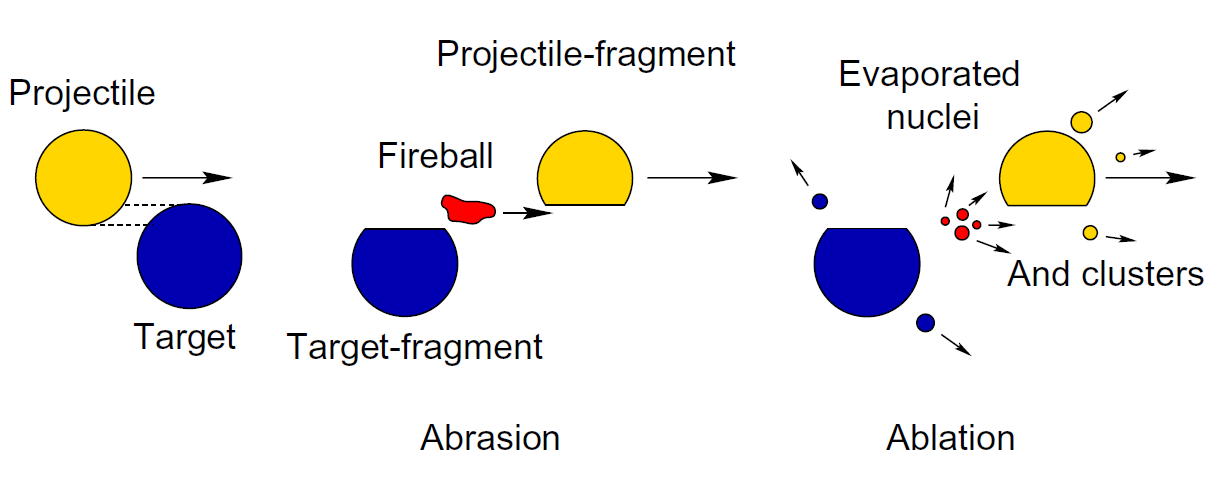
\includegraphics[width=0.8\textwidth]{images/ablationabration.png}  
\caption{Schematic of the physics involved.}
 \label{fig:ablationabration}
 \end{center}
 \end{figure}



\subsection{Simulation}

The simulation is to be performed with the latest versions of the INCL and ABLA code that is a part of the GEANT4 suite.

INCL is a monte Carlo simulation Intranuclear cascade model. INCL is developed from the on Liege cascade, but contains less free parameters in order to improve certain discrepancies in the Liege code.

dimdim needs to be expanded-


\begin{figure} 
\begin{center}
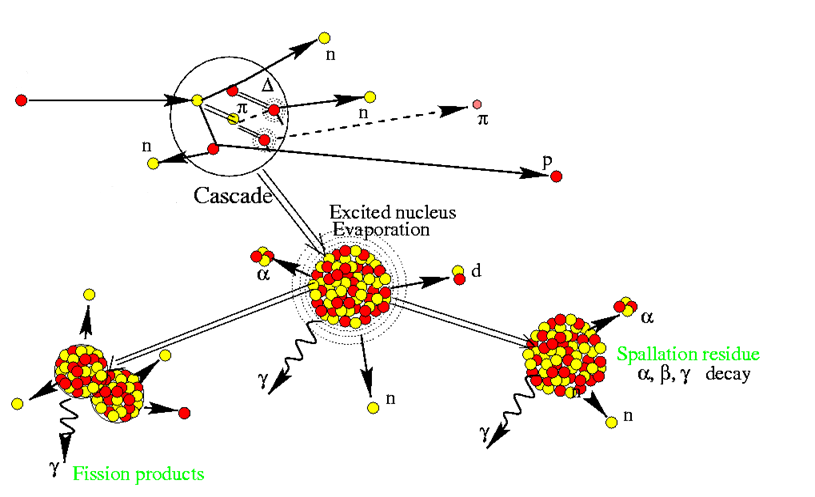
\includegraphics[width=0.8\textwidth]{images/inclScematic.png}  
\caption{\label{fig:inclschematic} Schematic diagram of INCL and ABLA models.}
 
 \end{center}
 \end{figure}
Particles penetrating matter do not just loose energy through inelastic collisions with the
target electrons, they might be involved in nuclear reactions and be fragmented. High
energy projectiles can be described as particles that move on straight lines through the
target and from time to time a target nucleus lies on this line and causes a collision. A
nuclear interaction model known as abrasion-ablation model uses this idealization. Projectile
and target nucleons which overlap in the collision process are called participants,
while the remaining parts of the projectile and target nucleus are called spectators. The
spectator projectile leaves the collision point with nearly unchanged velocity and direction,
while the target spectator stays at rest. The participant nucleons form an excited
complex called \reball", which breaks into single nucleons or light ions like , deuterons
and tritons.

\section{Simulation setup}
\begin{itemize}
\item Experiment data from GSI
\item target description
\item Characterization of the beam
\item Simulation of detectors
\item Implementation details
\end{itemize}

\section{Results and comparison to GSI data}
\begin{itemize}
\item comparison (Haettner 5.4.1)
\item energy distribution of fragments
\end{itemize}

\section{Conclusion}
\begin{itemize}
\item Raflaava yhteenveto
\end{itemize}

\section{Appendices}
\begin{itemize}
\item code examples
\item runtime log
\end{itemize}





\bibliographystyle{plain} \bibliography{refs.bib} 
\end{document}

\else

\fi